\documentclass[12pt, titlepage]{article}
\usepackage{../project_latex/report-style}


%------------------------------------------------------------------------------
%------------------------------------------------------------------------------
% Document Info
%------------------------------------------------------------------------------
%------------------------------------------------------------------------------
\newcommand{\docTitle}{Software Requirements Specification}
\newcommand{\dueDate}{October 6, 2017}


%------------------------------------------------------------------------------
%------------------------------------------------------------------------------
% Revision Table
%------------------------------------------------------------------------------
%------------------------------------------------------------------------------
\newcommand{\revisionTable}{
	\begin{table}[hp]
		\caption{\bf Revision History}
		\begin{tabularx}{\textwidth}{p{3cm}p{2cm}X}
			\toprule {\bf Date} & {\bf Version} & {\bf Notes}\\
			\midrule
			
			06-Oct-2017 & 0.0 & Revision 0\\
			
			\bottomrule
		\end{tabularx}
	\end{table}
}

\newcommand{\pbox}[1]{\parbox[t]{.85\linewidth}{#1}
}
\newcommand{\myline}{%\par
	\kern1pt % space above the rules
	%	\hrule height 1.5pt
	%	\kern2pt % space between the rules
	\hrule height 0.8pt
	\kern3pt % space below the rules
}
\newcommand{\requirement}[7]{

	\noindent
	\vspace{5pt}
	\parbox{\linewidth}{
		\fontsize{10pt}{5pt}\selectfont
		\noindent\textbf{#1} \hspace{26pt}\pbox{\textit{#2}} \\
		%		\hrule height 1pt
		\myline
		%		\parbox{0.7\linewidth}{
		\textit{Rationale:}	\hspace{10pt} \pbox{#3} \\
		\textit{Fit Criterion:} \pbox{#4} \\
		\textit{Priority:} \hspace{18pt} \pbox{#5} \\
		\textit{Originator:} \hspace{7pt} \pbox{#6} \\
		\textit{History:} \hspace{25pt}{#7} \\
}}



\newcommand{\labelWidth}{55pt}
\newcommand{\descWidth}{5.13in}

\newcommand{\pbox}[1]{\parbox[t]{\descWidth}{#1}}

\newcommand{\labelbox}[1]{\parbox[t]{\labelWidth}{\textit{#1}}}
\newcommand{\myline}{%\par
	\kern1pt % space above the rules
	%	\hrule height 1.5pt
	%	\kern2pt % space between the rules
	\hrule height 0.8pt
	\kern3pt % space below the rules
}


% Uncomment all between lines for new requirement macro
%-------------------------------------------------
%\newcommand\Tstrut{\rule{0pt}{0.5ex}}         % = `top' strut
%\newcommand\Bstrut{\rule[-0.9ex]{0pt}{0pt}}   % = `bottom' strut
%\newcounter{nfrCounter}
%
%% nonfunctional req
%\newcommand{\nfr}[7]{
%	\begin{center}
%		\noindent\vspace{5pt}
%		\refstepcounter{nfrCounter}
%		\fontsize{9pt}{5pt}\selectfont
%		
%		\parbox{\linewidth}{
%			\begin{tabular}[h]{l l}
%				\textbf{\textit{\labelbox{NFR\thenfrCounter}}} & \textit{\pbox{#1}} \\[2.5ex]
%				
%				\hline \\[-0.8ex]
%				
%				\labelbox{Rationale} & \pbox{#2} \\
%				\labelbox{Fit Criterion} & \pbox{#3} \\[6pt]
%				\labelbox{Priority} & \pbox{#4} \\
%				\labelbox{Originator} & \pbox{#5} \\
%				\labelbox{History} & \pbox{#6} \\
%				\hline
%			\end{tabular}
%		} \par 
%	\end{center}
%}

%%\requirement{arg1}{arg2}{arg3}{arg4}{arg5}{arg6}{arg7}\\
%\nfr{In order to accommodate as many users as possible, the user should be able to adjust the font size for the app.
%}{An application that is accessible to people with poor eyesight or other disabilities will increase the application’s potential user-base size.
%}{The user should not have to wait for more than 1 second for any operation to complete. If this is not possible due to network conditions, then there should be some kind of visible progress displayed to the user.
%}{Medium}{Dawson Myers}{October 6, 2017}
%-------------------------------------------------

\begin{document}
%------------------------------------------------------------------------------
%------------------------------------------------------------------------------
%	Title Page
%------------------------------------------------------------------------------
%------------------------------------------------------------------------------


\begin{titlepage}

%------------------------------------------------------------------------------
%------------------------------------------------------------------------------
%	Document Information
%------------------------------------------------------------------------------
%------------------------------------------------------------------------------

% Team Info
\newcommand{\teamname}{REST Assured}
\newcommand{\teamnumber}{Team 31}

% Project Info
\newcommand{\course}{SE 3XA3}

% \docTitle defined in main tex doc
\title{\course: \docTitle \\ \teamname}

% Student 1
\newcommand{\studentAname}{Dawson Myers}
\newcommand{\studentAsid}{400005616}
\newcommand{\studentAmid}{myersd1}
\newcommand{\studentAInfo}{\studentAname \studentAsid \studentAmid}

% Student 2
\newcommand{\studentBname}{Yang Liu}
\newcommand{\studentBsid}{400038517}
\newcommand{\studentBmid}{liuy136}
\newcommand{\studentBInfo}{\studentBname \studentBsid \studentBmid}

% Student 3
\newcommand{\studentCname}{Brandon Roberts}
\newcommand{\studentCsid}{400018117}
\newcommand{\studentCmid}{roberb1}
\newcommand{\studentCInfo}{\studentCname \studentCsid \studentCmid}


\author{\teamnumber
	\\ \teamname
	\\ \studentAInfo
	\\ \studentBInfo
	\\ \studentCInfo
	%\\ Dawson Myers 400005616  mysersd1
	%\\ Yang Liu 400038517 liuy136
	%\\ Brandon Roberts 400018117 roberb1
}

\date{\dueDate}


%\maketitle

\centering
\parbox[t]{0.97\linewidth}{
	\centering \fontsize{20pt}{25pt}\selectfont % The first argument for fontsize is the font size of the text and the second is the line spacing

	\Large \course \\
	\huge \teamname \\
	\large\dueDate
	
	\vspace{0.1in}
	\hrule
	\vspace{0.1in}
	
	\Huge \docTitle
	
	\vspace{0.05in}
	\hrule
	\vspace{0.4in}
	
	\large \teamnumber
	
	\vspace{0.1in}
}

% Team member info
%-------------------------------------------------------------------------------
\begin{minipage}[c]{\linewidth}
%\fontsize{14pt}{25pt}\selectfont
			\large
			\centering
			\begin{tabular}{l c c}
				\studentAname & \studentAmid & \studentAsid \\
				\studentBname & \studentBmid & \studentBsid \\
				\studentCname & \studentCmid & \studentCsid \\
			\end{tabular}
\end{minipage}

%\vfill

%% Revision table
%%-------------------------------------------------------------------------------
%\begin{table}[bp]
%	\caption{\bf Revision History}
%	\begin{tabularx}{\textwidth}{p{3cm}p{2cm}X}
%		\toprule {\bf Date} & {\bf Version} & {\bf Notes}\\
%		\midrule
%		
%		06-Oct-2017 & 0.0 & Revision 0\\
%
%		\bottomrule
%	\end{tabularx}
%\end{table}

%\revisionTable

\end{titlepage}


%------------------------------------------------------------------------------
%------------------------------------------------------------------------------
%	Report
%------------------------------------------------------------------------------
%------------------------------------------------------------------------------

\pagenumbering{roman}
\def\thesection{\arabic{section}} 
\renewcommand\thesection{\arabic{section}} 
\renewcommand\thesubsection{\thesection.\arabic{subsection}}

\tableofcontents

\listoftables

\listoffigures


\newpage

\pagenumbering{arabic}
%==============================================================================
\section{Revision History}
%==============================================================================
\revisionTable

This document describes the requirements for the REST client testing tool. The template for the Software
Requirements Specification (SRS) is a subset of the Volere template~\citep{RobertsonAndRobertson2012}.

%==============================================================================
\section{Project Drivers}
%==============================================================================



\subsection{The Purpose of the Project}
%------------------------------------------------------------------------------
Web services developed using web application programming interface (API) are omnipresent. Web APIs offers a powerful platform that enables HTTP services to a broad range of clients including browsers, mobiles, and desktops. They are created based on the representational state transfer (REST) framework that presents guidelines acting as a standard for Web APIs. It is critical to be able to test the API functionalities during its development stage. The reconstruction of the Sails Live Chrome app will provide software developers a tool in Web API building and testing. The application will provide tests endpoints and the capability to diagnose bugs in applications featuring RESTful interfaces.

\subsection{The Stakeholders}
%------------------------------------------------------------------------------
Stakeholders include the project team members developing the project who are learning about the software engineering project development process and the McMaster University Software Engineering 3XA3 course teaching staff who are invested in the educational value of the project for the development team. The product is not developed for commercial sale to customers, but rather as an open source utility tool free to developers who see a need for it. Therefore, the team itself is putting their own resources into the project.

\subsubsection{The Client}
%------------------------------------------------------
The client is Professor Asghar Bokhari who is teaching the McMaster University Software Engineering 3XA3 course. Since the project is intended to be open source and the core project team sets the project direction, desired features and software requirements for the product, they may be considered as both the clients and the stakeholders.

\subsubsection{The Customers}
%------------------------------------------------------
The customers are developers who have a need for a REST client for testing their app. However, there app is a free utility, so they will not be paying customers.

\subsubsection{Other Stakeholders}
%------------------------------------------------------
Given the limited scope of the project, there are no other stakeholders beyond what has been listed above.

\subsection{Mandated Constraints}
%------------------------------------------------------------------------------
\subsubsection{Solution Constraints}

The product shall operate on up-to-date versions of Windows, Mac, Linux operating systems with up-to-date versions of Chrome browsers installed that allow JavaScript to run. Rationale: Target client are users of up-to-date Windows, Mac, Linux operating systems with JavaScript client. 


The product shall operate with a working and secure Internet connection with a download speed above 5 Mbps and an upload speed above 1 Mbps. The desired Internet connection speed is directly proportional to the quantity of data clients require for the testing of their specific web APIs (higher Internet connection speed is desired for applications with higher data traffic).
Rationale: The product uses Internet connection to serve REST requests to required resources and to display request responses.

The product shall comply with Canadian federal privacy laws (Privacy Act and Personal Information Protection and Electronic Documents Act) and other relevant legal requirements. Rationale: The product should not breach legal requirements in the intended operating environment.


\subsubsection{Off-the-Shelf Software}
The execution of product requires the following off-the-shelf software:
\begin{itemize}
	\item Google Chrome web browser
	\item Client on which Chrome apps can be installed  
	\item JavaScript
\end{itemize}
All of the above are freely available on the Internet.

\subsubsection{Schedule Constraints}
A working product must be completed to a state demonstrating full functionality for final demonstration by Nov 27, 2017. The product shall be completed for product release (along with all final documentation) by Dec 6, 2017.

\subsubsection{Budget Constraints}
The expected operation budget for the product is \$0, thus requirements for purchasing materials and other product needs are not applicable. Any unplanned purchases and costs during the development process are expected to be covered by the project team out of pocket.

\subsubsection{Enterprise Constraints}
The product is open-source and therefore freely accessible to all users with the technology and platform to run Chrome applications and JavaScript.

\subsection{Naming Conventions and Terminology}
%------------------------------------------------------------------------------
\begin{itemize}
	\item HTTP: Hypertext Transfer Protocol.
	\item REST: Representational state transfer (REST) or RESTful web services is a way of providing interoperability between computer systems on the Internet.
	\item JSON: JavaScript Object Notation. An open-standard file format that uses human-readable text to transmit data objects consisting of attribute–value pairs and array data types (or any other serializable value).
	\item API: Application Program Interface. A document detailing the name of each function the client may call in their software and the purpose of those functions.
	\item Functional Requirements: Requirements that describes what the product will do.
	\item User: A person who will be using the final product.
	\item App: The application being designed; the system-to-be.
\end{itemize}


\subsection{Relevant Facts and Assumptions}
%------------------------------------------------------------------------------
It is assumed that the users will be software developers with a basic understanding of REST interfaces and the HTTP protocol.

\newpage
%==============================================================================
\section{Functional Requirements}
%==============================================================================

\subsection{The Scope of the Work and the Product}
%------------------------------------------------------------------------------
\begin{center}
	\begin{figure}[h!]
		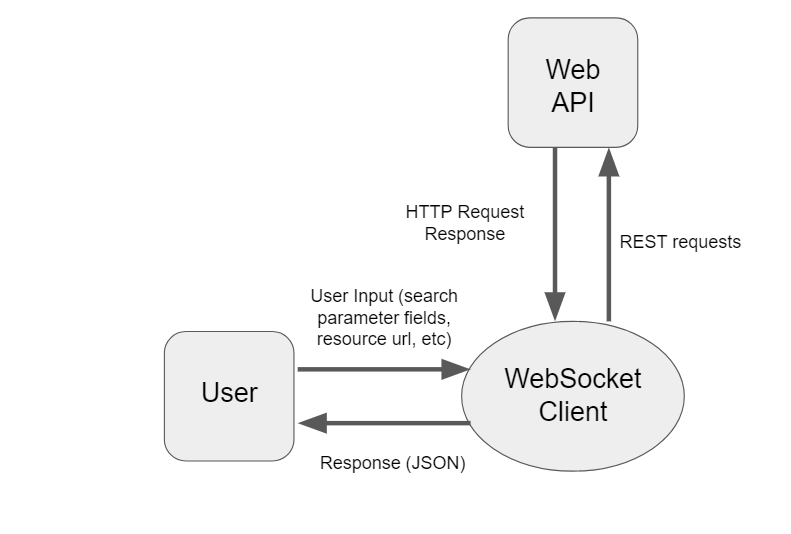
\includegraphics[width=1\linewidth, center]{images/srs-io-dia}
		\caption{Context Diagram}
	\end{figure}
\end{center}
\subsubsection{The Context of the Work}
%------------------------------------------------------
The recreation of the app is not limited to any particular platform since most devices are able to support the Chrome web browser and run JavaScript. The reproduction of the app will remove the limitation presented by Sails Live that users can interface with only the Sails server. Instead, the reproduced app aim to enable communication with interfaces featuring RESTful Web APIs not limited to Sails.

\subsubsection{Work Partitioning}
%------------------------------------------------------
Not relevant for this project.

\subsubsection{Individual Product Use Cases}
%------------------------------------------------------
Figure \ref{image:usecase} shows a use case for the app.

\begin{center}
	\begin{figure}[h!]
		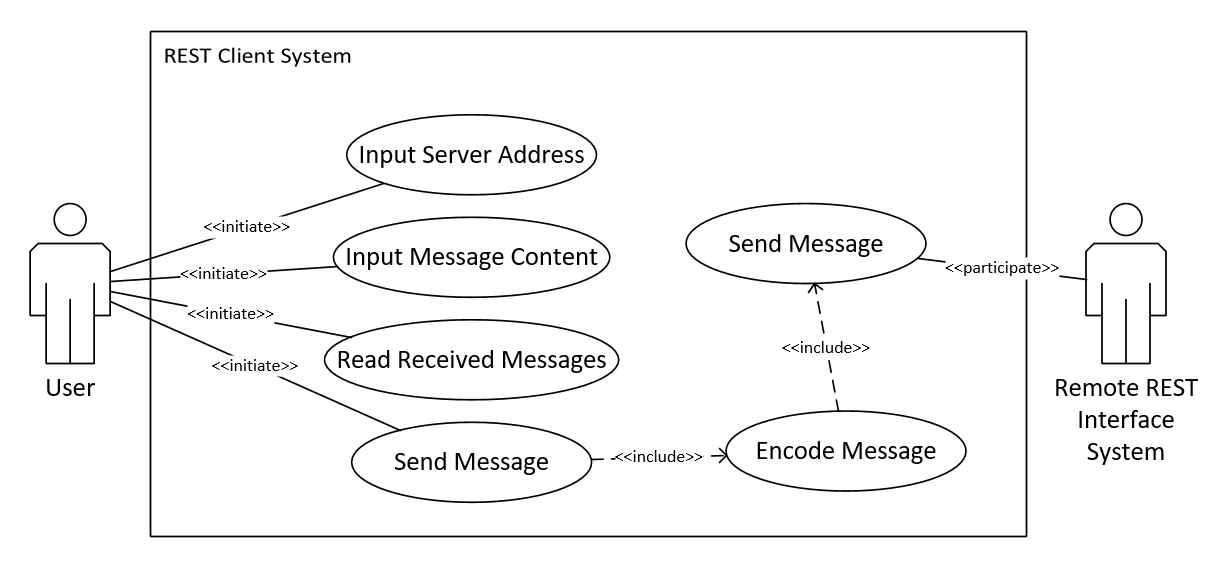
\includegraphics[width=0.8\linewidth, center]{images/srs-use-case-send-msg}
		\caption{Send Message Use Case Diagram}
		\label{image:usecase}
	\end{figure}
\end{center}


\subsection{Functional Requirements}
%------------------------------------------------------------------------------
\begin{enumerate}
	\item[FR1] The app shall be able send and receive HTTP messages.
	\item[FR2] Message format shall strictly follow the REST communication protocol.
	\item[FR3] The app must provide a user interface that allows users to view the content of sent and received messages.
	
\end{enumerate}
%==============================================================================
\section{Non-functional Requirements}
%==============================================================================


%\requirement{arg1}{arg2}{arg3}{arg4}{arg5}{arg6}
\subsection{Look and Feel Requirements}
%------------------------------------------------------------------------------
\requirement{NFR1}{The app should have a simplistic and intuitive user interface.}
{An application that is easy to use will make it more accessible to users. It will also increase productivity.}
{At least 90\% of users should be able to use the user interface to connect to a REST endpoint within 5 minutes of use.}{High}{Dawson Myers}{October 6, 2017}

\requirement{NFR2}{
The app should be easy to install.
}{95\% of users should be able to locate and install the app via the Chrome App Store without encountering issues.
}{Apps that are easy to install are more likely to be used.
}{High}{Dawson Myers}{October 6, 2017}

	
\subsection{Usability and Humanity Requirements}
%------------------------------------------------------------------------------
\requirement{NFR3}{In order to accommodate as many users as possible, the user should be able to adjust the font size for the app.
}{An application that is accessible to people with poor eyesight or other disabilities will increase the application’s potential user-base size.
}{The user should not have to wait for more than 1 second for any operation to complete. If this is not possible due to network conditions, then there should be some kind of visible progress displayed to the user.
}{Medium}{Dawson Myers}{October 6, 2017}

\subsection{Performance Requirements}
%------------------------------------------------------------------------------

\requirement{NFR4}{The user interface should be responsive to user actions and not appear to be slow or hung up during normal operation.
}{An application that responds quickly to the user leads to an overall more positive reception.
}{The user should not have to wait for more than 1 second for any operation to complete. If this is not possible due to network conditions, then there should be some kind of visible progress displayed to the user.
}{Medium}{Dawson Myers}{October 6, 2017}
\subsection{Operational and Environmental Requirements}
%------------------------------------------------------------------------------
\requirement{NFR5}{The app should be able to run on any system that Google Chrome can run on.
}{Google Chrome is offered on almost every operating system. Running the application through Google Chrome will maximize the app’s potential.
}{The app should be compatible with Windows, Linux, and Mac OS.
}{Medium}{Dawson Myers}{October 6, 2017}
\subsection{Maintainability and Support Requirements}
%------------------------------------------------------------------------------
\requirement{NFR6}{The app should be able to be updated on users machines in a simple, unintrusive and automated fashion.
}{ Keeping the application up-to-date in a simple, unintrusive and automated fashion is convenient and desirable for the end user.
}{The app should utilize the updating mechanism that is used by the Chrome App Store.
}{Medium}{Dawson Myers}{October 6, 2017}
\subsection{Security Requirements}
%------------------------------------------------------------------------------
\requirement{NFR7}{The app should not, in any way, access private data on users’ computers.
}{Accessing a user’s private information without express consent is a violation of the law. Therefore, the application will never access private information this without consent.
}{Users must first give consent before any data is accessed by the app.
}{Medium}{Dawson Myers}{October 6, 2017}

\requirement{NFR8}{The app should not make users’ computers vulnerable to any cyber threats.
}{Protecting the user’s machine from external threats is important, and is mandated by the law in Canada.
}{The app must not allow any form of remote access or subvert the cyber defence mechanisms on the host computer.
}{High}{Dawson Myers}{October 6, 2017}

\subsection{Cultural Requirements}
%------------------------------------------------------------------------------
\requirement{NFR9}{The app should not be offensive to users.
}{Offensive material could lower productivity, or turn away potential users.
}{The app should not be offensive to at least 85\% of potential users. The application will launch without any material perceived offensive by team members.
}{High}{Dawson Myers}{October 6, 2017}

\requirement{NFR10}{The app should be understandable to users that understand english, regardless of culture.
}{Lack of cultural images and references makes it easier for users to understand the uses of the application.
}{The app should not contain any cultural images or references.
}{Medium}{Dawson Myers}{October 6, 2017}
\subsection{Legal Requirements}
%------------------------------------------------------------------------------
%\requirement{NFR9}{
%}{
%}{
%}{Medium}{Dawson Myers}{October 6, 2017}

The application must not take personal information from the user without their express consent, in accordance with relevant Canadian and US laws. The app must not infringe on any copyright, trademarks, or intellectual properties.

\subsection{Health and Safety Requirements}
%------------------------------------------------------------------------------
Health and safety are issues that should be considered for every engineering project. The product does not interact with users physically and thus do not impose physical health concerns to the users. Safety precautions should be taken to protect the privacy of users and safeguard any personal information. The product requirements and constraints taken into consideration that the product must abide by all Canadian federal privacy laws to achieve this standard.

%==============================================================================
\section{Project Issues}
%==============================================================================

\subsection{Open Issues}
%------------------------------------------------------------------------------
There are currently no open issues.

\subsection{Off-the-Shelf Solutions}
%------------------------------------------------------------------------------
Some off-the-shelf solutions that will be utilized for app include JavaScript frameworks such as Angular and jQuery.

\subsection{New Problems}
%------------------------------------------------------------------------------
Data storage is currently being discussed and will likely have an issue opened for it soon. The issue involves the format for storing configuration data on host machines.
\subsection{Tasks}
%------------------------------------------------------------------------------
The tasks for the project is set forth by the McMaster University Software Engineering 3XA3 course deliverables outline.\\

\subsubsection{Project Planning}
The project will follow the schedule in shown in table \ref{table:projsched}.
	\begin{table}[h]
		\begin{center}
	\begin{tabular}{||c c c||} 
		\hline
		Task Item & Revision & Timeline \\ [0.5ex] 
		\hline\hline
		Proof of Concept Demonstration & 0 & Oct 16, 2017 \\ 
		\hline
		JavaScript Design &  0 & Oct 20, 2017 \\
		\hline
		JavaScript Implementation &  0 & Oct 25, 2017 \\
		\hline
		Test Plan & 0 & Oct 27, 2017 \\
		\hline
		Design Document &  0 & Nov 10, 2017 \\
		\hline
		Revision 0 Demonstration & 0 & Nov 13, 2017 \\
		\hline
		Final Demonstration & 1 & Nov 27, 2017 \\
		\hline
		Final Documentation & 1 & Dec 6, 2017  \\ [1ex] 
		\hline
	\end{tabular}
	\caption{Project Schedule}
	\label{table:projsched}
\end{center}
	\end{table}


\subsection{Migration to the New Product}
%------------------------------------------------------------------------------
Not applicable to this project.

\subsection{Risks}
%------------------------------------------------------------------------------
One risk factor involved with the project is that automated testing may be difficult to implement due to variation in request responses to applications featuring live outputs (such as Twitter API). The project has been through a preliminary round of evaluation by the teaching staff of the course to ensure the planned scope has maximum potential for project success. However, in case the scope of the project is too large to complete within the designated project time line, there may be need to narrow the scope of the project to allow project completion.

\subsection{Costs}
%------------------------------------------------------------------------------
The product is projected to incur no monetary cost as long as services such as source code hosting and version control systems are free of cost to the project team. The main cost is the time of the project team members who develop and maintain the product.

\subsection{User Documentation and Training}
%------------------------------------------------------------------------------
It is important for users to learn how to use the application. Simple annotated screen shots will be provided to explain how to use the basic functions of the application.

\subsection{Waiting Room}
%------------------------------------------------------------------------------
Features that are considered for future releases include:
\begin{itemize}
	\item Socket connection support for remote applications and interfaces 
	\item Real-time payload validation (JSON validation)
	\item Request management (edit, remove, sort or inspect created requests)
	\item Event registration (on which the connected socket should listen to)
	\item Create, manage and inspect listeners
	\item Observe realtime notifications
	\item Collapsable response inspector
	\item Listener queue (list and save all incoming events with date and time information)
	\item Multiple connections (select the socket you need for each request and listener)
	\item Connection history
	\item Automated API tests with configuration
	\item Import/Export of custom settings
\end{itemize}
\subsection{Ideas for Solutions}
%------------------------------------------------------------------------------
Stated in previous sections.

\bibliographystyle{plainnat}

\bibliography{SRS}

\newpage

%==============================================================================
\section{Appendix}
%==============================================================================
This section has been added to the Volere template.  This is where you can place
additional information.

\subsection{Symbolic Parameters}
%------------------------------------------------------------------------------

Symbolic parameters are yet to be determined.


\end{document}